\parindent=0em
\subsection{Educación}
\noindent

%https://www.microsoft.com/es-es/education/mixed-reality
Las tecnologías inmersivas están ganando popularidad y haciéndose más accesibles para los consumidores, esto está provocando que se empiece a usar en sectores como la educación. Aunque está aumentando el consenso entre expertos de que dichas tecnologías hacen una gran aportación a la educación en forma de motivación y, una manera innovadora de aprender para los estudiantes, no existe un léxico común ya que los expertos redefinen constantemente los términos en este campo. Alice Bonasio \cite{microsoftEducation} afirma que la realidad mixta ofrece los siguientes beneficios en la educación:

\begin{itemize}
    \item \textbf{Proceso cognitivo:} La realidad mixta ofrece un entorno seguro para practicar y perfeccionar habilidades, reduce los cuellos de botella debidos al exceso de información y mejora el desempeño en tareas basadas en habilidades. Esto da lugar a un mayor aprendizaje, razonamiento abstracto y pensamiento crítico, además, está demostrado que los resultados de los alumnos mejoran un 22\% al hacer uso de esta tecnología. 
    
     \item \textbf{Acogida social y aprendizaje emocional:} Ya que el precio de estas tecnologías está disminuyendo permite a algunos estudiantes el acceso a experiencias inalcanzables para ellos anteriormente. La realidad mixta permite configuraciones colaborativas y pone a los estudiantes en la perspectiva de otras personas, favoreciendo las habilidades relacionadas con la empatía.
     
     \item \textbf{Comportamiento:} Las simulaciones permiten a los usuarios practicar situaciones rutinarias o acceder a experiencias que serían inalcanzables en el mundo real. Los estudiantes que aprenden a través de la realidad mixta presentan un mayor nivel de concienciación con el entorno, normalmente llevándoles a un cambio concreto de comportamiento, asimismo, se aprecian mejorías en las habilidades de los alumnos para aplicar conceptos teóricos aprendidos en escenarios del mundo real.
\end{itemize}

En conclusión, la realidad mixta en el ámbito de la educación reduce la carga cognitiva, aumenta la retención de conocimientos y desencadena la empatía.\\


%https://www.microsoft.com/es-es/p/vr-frog-dissection-ribbit-ing-discoveries/9mvjk426cbt1?CustomerIntent=Consumer&activetab=pivot%3Aoverviewtab#


Por otro lado, empresas como Microsoft ofrecen distintas aplicaciones vinculadas a su plataforma Windows Mixed Reality para fomentar la educación, por ejemplo, \textit{VR Frog Dissection: Ribbit-ing Discoveries} (figura \ref{fig:vrfrogdissectioncapturas}) una experiencia de realidad mixta (pese a su título) a través de la cual los usuarios pueden aprender cómo se disecciona una rana.

\begin{figure}[htbp]
\centering
    \hspace{-4mm}
    \begin{minipage}{0.5\textwidth}
        \centering
        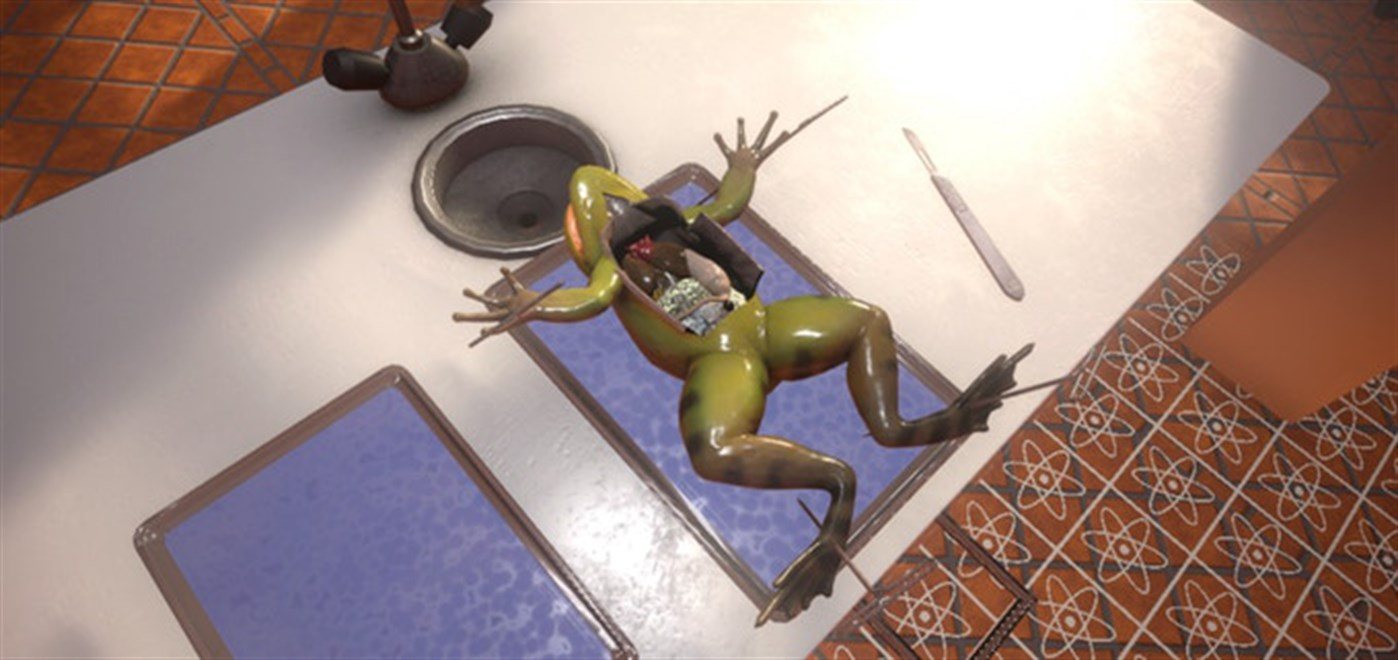
\includegraphics[scale=0.16]{Images/Estado del arte/frogDisection1.jpeg}\\
    \end{minipage}
    \begin{minipage}{0.5\textwidth}
        \centering
        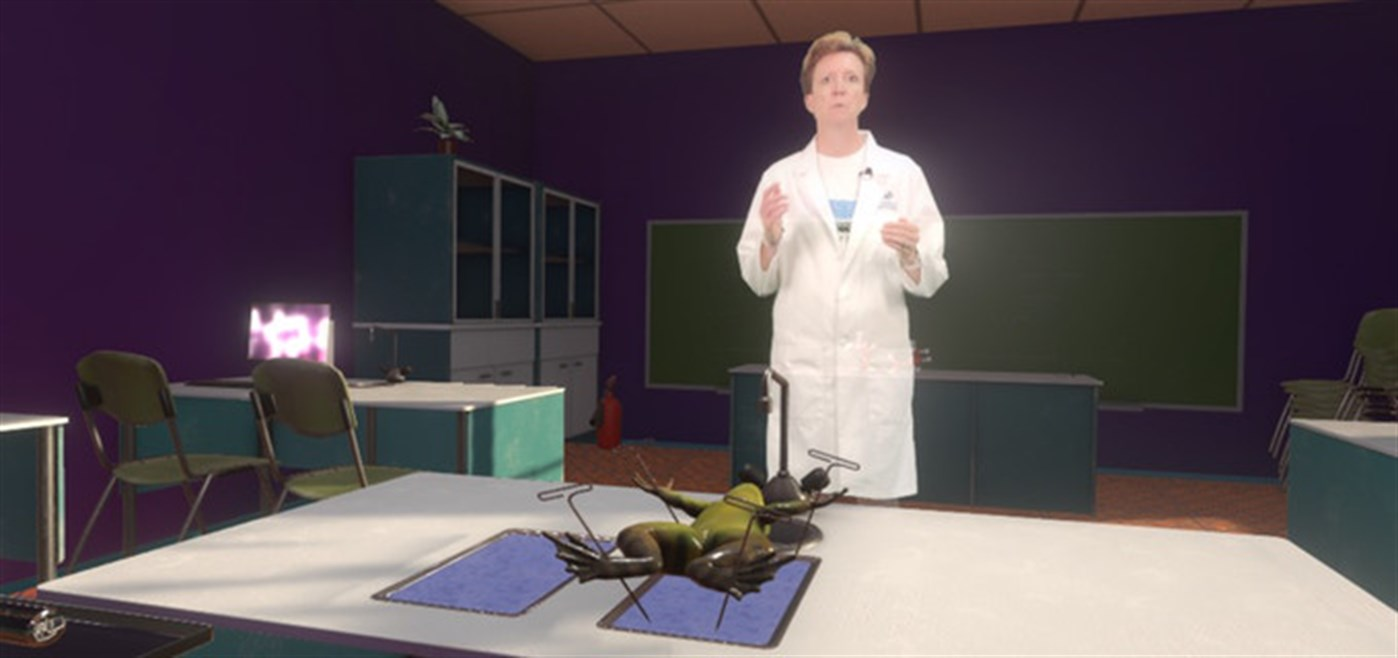
\includegraphics[scale=0.16]{Images/Estado del arte/frogDisection2.jpeg}\\
    \end{minipage}\\
    \caption{Capturas del juego VR Frog Dissection: Ribbit-ing Discoveries}
    \label{fig:vrfrogdissectioncapturas}
\end{figure}

Otras de las muchas experiencias que nos ofrece esta plataforma de Microsoft son \textit{HoloTour} (una combinación de vídeo de 360 grados, sonido espacial y paisajes holográficos) o la aplicación de navegación 3D a través del cuerpo humano llamada \textit{Holo-Human}. Se puede usar esta experiencia de forma colaborativa para descubrir la anatomía de un cuerpo humano (figura \ref{fig:capturaHoloHuman}).

\begin{figure}[h]
    \centering
    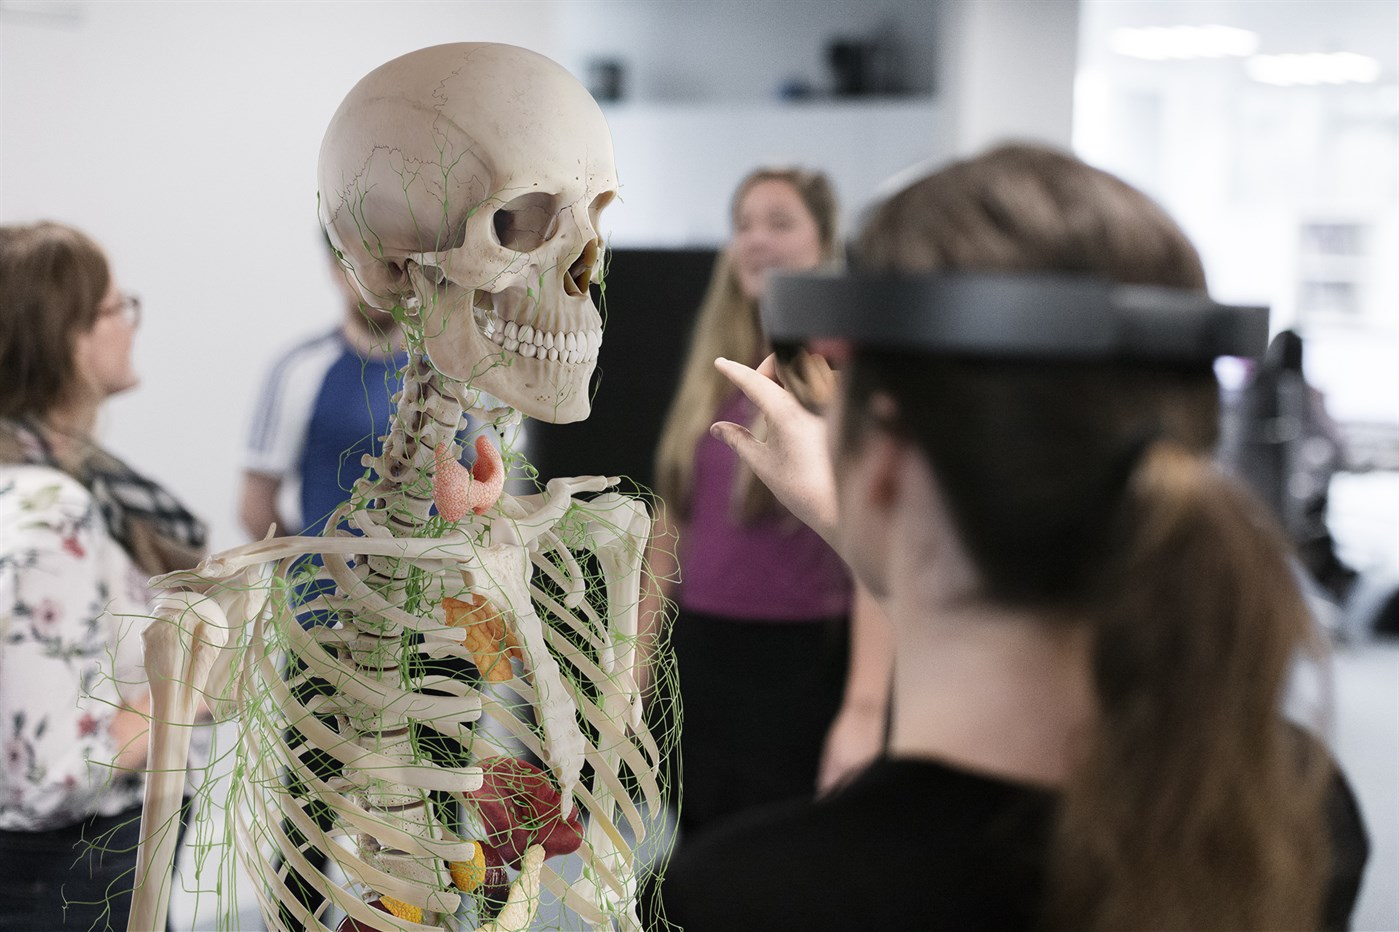
\includegraphics[scale=0.25]{Images/Estado del arte/holohuman.jpeg}
    \caption{Captura de la aplicación \textit{Holo-Human}}
    \label{fig:capturaHoloHuman}
\end{figure}

%https://www.microsoft.com/es-es/p/holo-human/9pggbknrbckj?CustomerIntent=Consumer&activetab=pivot%3Aoverviewtab#

